\subsection{Competition results}
The competition took place on two dates (15th and 17th of September) and each team had to play three times against all other teams. Each simulation consisted of a total of 400 steps and the team with the highest score at the end got three points for a victory. The overall score is the sum over all 400 step scores. The score per step is composed of points for zones plus achievement points. Since the strategy of team "MaKo" was to extensively buy upgrades for the artillery agent", most of the earned achievement points were consumed and therefore did not count towards the step score. Figure \autoref{dis:achievement_points} shows the progress of achievement points over time. As one can see, the achievement points of team "MaKo" go up and down due to the buying actions whereas the the points of the other team increase constantly. 
\begin{figure}[ht]
	\centering
	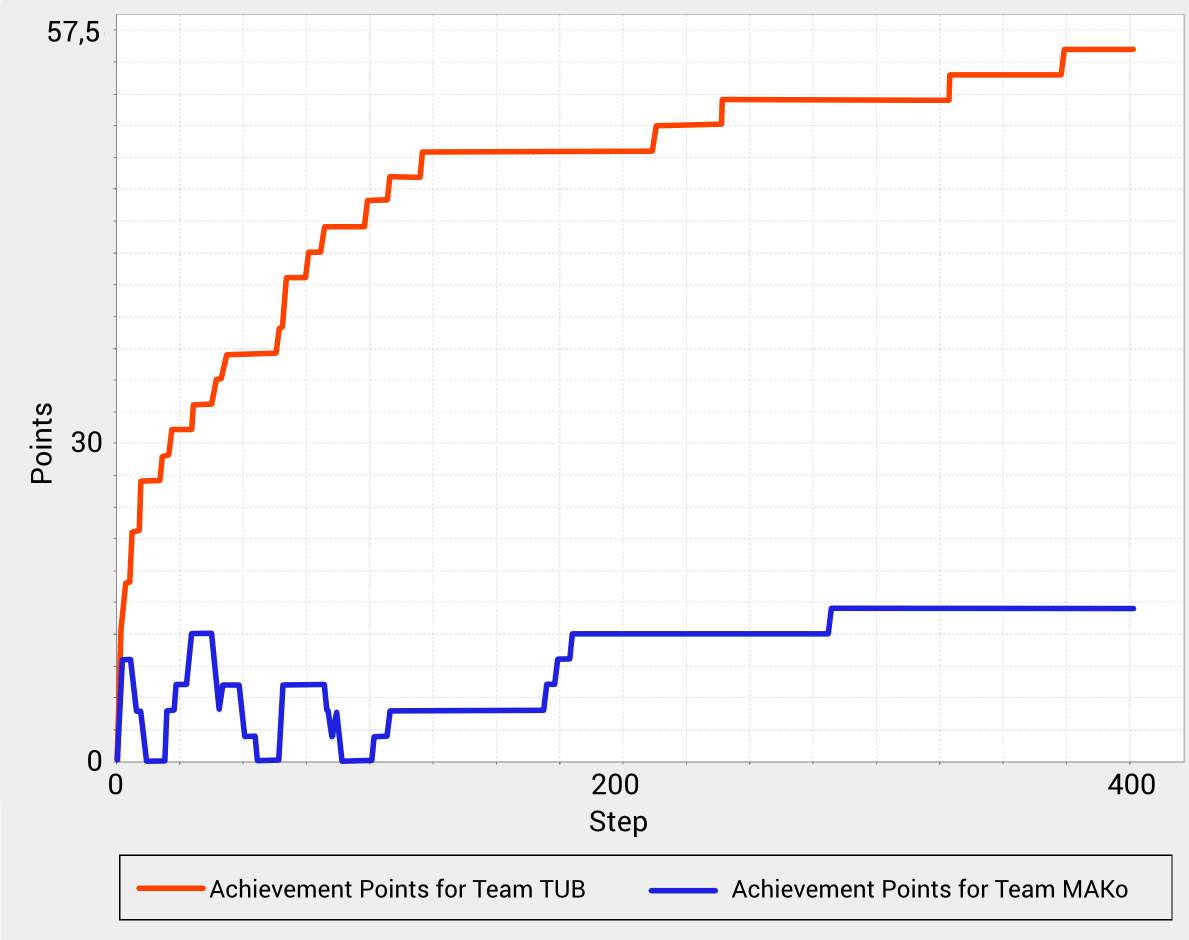
\includegraphics[width=300px]{images/AchievementPoints.png}
	\caption{MAPC 2014 result}
	\label{dis:achievement_points}
\end{figure}
It looks like that this is a huge drawback because achievement points earned at some point count into every future step score. But compared to the number of points awarded for zones, this is only a minor fraction of the step score. As it can be seen in figure \autoref{dis:ZonesScoresAndAchievementPoints} the spending of achievement points paid off since our upgraded saboteur agents hindered the enemy agents from building high valued zones. It was worth spending the achievement points for the purpose of attacking and disturbing the other team because the amount of potential zone points they would have earned without being attacked, is probably much higher than the amount of achievement points team "MaKo" spent for upgrades.
\begin{figure}[h]
	\centering
	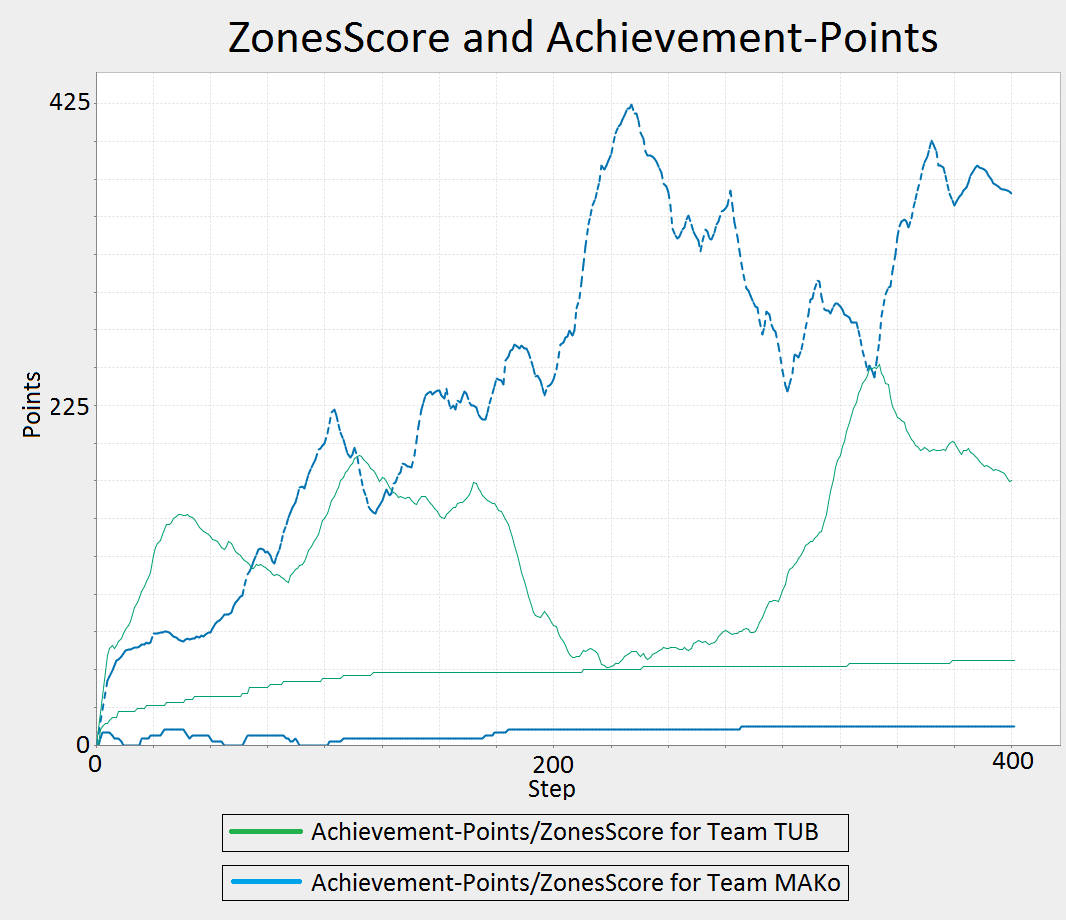
\includegraphics[width=300px]{images/ZonesScoresAndAchievementPoints.png}
	\caption{MAPC 2014 result}
	\label{dis:ZonesScoresAndAchievementPoints}
\end{figure}
At the end of the tournament team "MaKo" scored second with a total of 18 points. The winner 2014 was, for three times in a row now, the team from the USFC. The final results are shown in~\autoref{tab:mapc2014results}.
\begin{table}[ht]
\centering
\caption{The results of the 2014 MAPC. Each team fought three matches against every other team, and winning a match awarded 3 points.}
\label{tab:mapc2014results}
\begin{tabular}{@{}lllll@{}}
\toprule
Pos. & Team name      & Score            & Difference            & Points \\ \midrule
1    & SMADAS-UFSC    & 1180662 : 654624 & \phantom{-}526038     & 33     \\
2    & MAKo           & 617086 : 776868  & -15782                & 18     \\
3    & TUB            & 904874 : 872399  & \phantom{-}32475      & 15     \\
4    & TheWonderbolts & 711001 : 1014669 & -303668               & 15     \\
5    & GOAL-DTU       & 653178 : 748241  & -95063                & 9      \\ \bottomrule
\end{tabular}
\end{table}
Statistics of all the individual games can be found in the appendix.[reference here!!!!]

Team "MaKo" lost every second game against each opponent due to the fact that for some reason the repairer agents weren't able to repair. The reason behind this was not obvious to the team. Summarizing the matches, team "MaKo" was capable of exploring the map, building local optima zones, dealing with disabled agents and attacking the opponent. A thing that could be improved is the zoning behaviour. Due to the fact that zones were broken up on a regular basis, zones with a high value sometimes were discarded even when there was no need to do that. Also no handling of edge cases has been implemented which could improve zoning in the sense that the actual number of agents needed to build that zone could be less than the number calculated by our algorithm. Like already mentioned a strategy that worked out well, was the approach to upgrade the visibility range and the strength of one saboteur agent significantly. In all matches the it was able to disable enemy agents many times and therefore disturb zones and keep the enemy repairers busy, which kept them away from building zones. 

% TODO: these are from the TOC:
%What place did we rank? How did the others do? Analyse our matches shortly and point out problems we faced, how we tackled them and point out what had gone well.
